\documentclass{article}
\usepackage[utf8]{inputenc}
\usepackage{graphicx}
\usepackage{ragged2e}

\title{Problem 3 : Gaussian Integral (N3)}
\begin{document}

\maketitle

\centering\textbf{Persona}

\begin{figure}[htp]
    \centering
    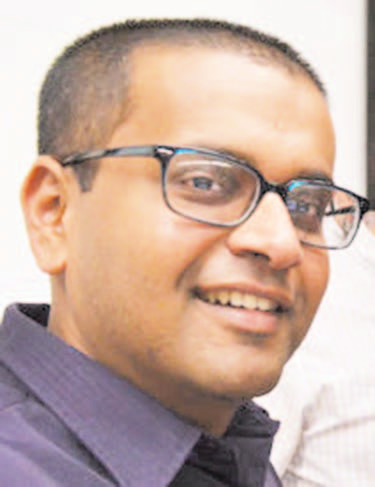
\includegraphics[width=4cm]{adhish}
\end{figure}
\textbf{Name : } Adhish Raval \hfill\break
\textbf{Age : } 32 \hfill\break
\textbf{Gender : } Male \hfill\break

\justifying
\noindent
\textbf{Background:} 
Bachelors in Science, Master in Physics, Doctor of Philosophy in Physics, working as a Researcher and a Professor at Sardar Vallabhbhai National Institute of Technology, Surat, India. \hfill\break

\justifying
\noindent
\textbf{Bio:}
Adhish is a physicist based in India, who is very passionate about his ongoing research in the field of Plasma Physics. He has also been teaching undergraduate students. Owing to his field, he learned many programming languages and even enjoys coding. He was interested in the field of Physics since he was in his Bachelors. He was very passionate about knowing the reason behind every phenomena in the universe. He does photography to de stress himself. He loves to be with nature, and firmly believes that nature is the best teacher. \hfill\break 

\justifying
\noindent
\textbf{Goals:} Adhish wishes to dig deeper into the field of Plasma physics and aims to find unknown answers to some of the most gravest questions of the universe which still remain unanswered. \hfill\break

\justifying
\noindent
\textbf{Strong suites:} Avid observer, Critical thinker, Passionate  and inquisitive physicist. \hfill\break

\justifying
\noindent
\textbf{Needs:}
\begin{itemize}
\item Adhish needs to do many complex calculations during his research.
\item Complex software to do calculations that requires accurate analysis of various concepts of calculus.
\item  Needs his students to have scientific calculators with them whenever they are working on physics numericals. \hfill\break
\end{itemize}
\justifying
\noindent   
\textbf{Frustrations:}   
\begin{itemize}
\item Teach students to use the scientific calculator
\item Search for values of various constants, widely used in the field of advanced mathematics and physics, on the internet. \hfill\break
\end{itemize}

\justifying
\noindent
\textbf{Environments:}
\begin{itemize}
\item Research laboratories
\item Personal office
\item University premises
\item Classrooms
\end{itemize}

\hfill\break

\end{document}
